\subsection{构建$C-C$段实体}
\begin{procedure}
\item 将视图方向切换为左视图,并绘制中心辅助线
\begin{lstlisting}
|命令: XLINE|
|指定点或 [水平(H)/垂直(V)/角度(A)/二等分(B)/偏移(O)]:|
|指定通过点:$ @1<0$|
|指定通过点:$ @1<90$|
|指定通过点:|
\end{lstlisting}
\item 绘制十字体

偏移产生十字线
\begin{lstlisting}
|命令: OFFSET|
|当前设置: 删除源=否  图层=源  OFFSETGAPTYPE=0|
|指定偏移距离或 [通过(T)/删除(E)/图层(L)] $<$5.0000$>$:  2|
|选择要偏移的对象,或 [退出(E)/放弃(U)] $<$退出$>$:|
|指定要偏移的那一侧上的点,或 [退出(E)/多个(M)/放弃(U)]$<$退出$>$:|
|选择要偏移的对象,或 [退出(E)/放弃(U)] $<$退出$>$:|
|指定要偏移的那一侧上的点,或 [退出(E)/多个(M)/放弃(U)]$<$退出$>$:|
|选择要偏移的对象,或 [退出(E)/放弃(U)]$<$退出$>$:|
|指定要偏移的那一侧上的点,或 [退出(E)/多个(M)/放弃(U)]$<$退出$>$:|
|选择要偏移的对象,或 [退出(E)/放弃(U)]$<$退出$>$:|
|指定要偏移的那一侧上的点,或 [退出(E)/多个(M)/放弃(U)]$<$退出$>$:|
|选择要偏移的对象,或 [退出(E)/放弃(U)] $<$退出$>$:|
\end{lstlisting}
因$F-F$段的十字形与此段的十字形结构基本相同,可以重复使用,因此以$\phi 46$圆做为基础。
\begin{lstlisting}
|命令: CIRCLE|
|指定圆的圆心或 [三点(3P)/两点(2P)/切点、切点、半径(T)]:|
|指定圆的半径或 [直径(D)] <15.5000>: 23|
\end{lstlisting}
修剪完成十字形(命令提示省略),结果如图\ref{fig:fabanc-c1}所示。
\begin{figure}[htbp]
\centering
\begin{floatrow}[3]
\ffigbox{\caption{修剪结果}\label{fig:fabanc-c1}}{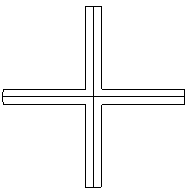
\includegraphics[scale=0.5]{fabanc-c1.png}}
\ffigbox{\caption{拉伸十字}\label{fig:fabanc-c2}}{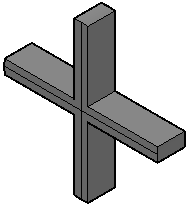
\includegraphics[scale=0.5]{fabanc-c2.png}}
\ffigbox{\caption{减去$\phi 42$圆柱}\label{fig:fabanc-c3}}{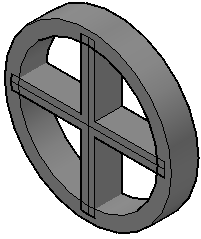
\includegraphics[scale=0.5]{fabanc-c3.png}}
\end{floatrow}
\end{figure}

\newpage
面域十字形。
\begin{lstlisting}
|命令: REG REGION|
|选择对象: 找到 12 个|
|选择对象:|
\end{lstlisting}
切换视图方向为西南等轴测,拉伸构建十字体,其结果如图\ref{fig:fabanc-c2}所示。

\begin{lstlisting}
|命令: EXTRUDE|
|当前线框密度:  ISOLINES=4,闭合轮廓创建模式 = 实体|
|选择要拉伸的对象或 [模式(MO)]: 找到 1 个|
|选择要拉伸的对象或 [模式(MO)]:|
|指定拉伸的高度或 [方向(D)/路径(P)/倾斜角(T)/表达式(E)]: -8|
\end{lstlisting}
将十字体及中心辅助线一起复制一份备用。复制命令的启动方法有:
\begin{itemize}
\item 键盘输入COPY或CO。
\item 点击【修改】菜单中的【复制】项
\item 点击【修改】工具栏中的【复制】图标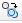
\includegraphics[scale=0.6]{copy.png}
\end{itemize}
\begin{lstlisting}
|命令: COPY|
|选择对象: 指定对角点: 找到 3 个|
|选择对象:|
|当前设置:  复制模式 = 多个|
|指定基点或 [位移(D)/模式(O)] $<$位移$>$: int 于|
|指定第二个点或 [阵列(A)] $<$使用第一个点作为位移$>$:|
|指定第二个点或 [阵列(A)/退出(E)/放弃(U)] $<$退出$>$:|
\end{lstlisting}
\item 以十字体辅助线的交点为圆心,绘制$\phi 50$圆柱体。
\begin{lstlisting}
|命令:  CYLINDER|
|指定底面的中心点或 [三点(3P)/两点(2P)/切点、切点、半径(T)|
|/椭圆(E)]:int 于|
|指定底面半径或 [直径(D)]: 25|
|指定高度或 [两点(2P)/轴端点(A)]$<$-8.0000$>$: |
\end{lstlisting}
\item 以十字体辅助线的交点为圆心,绘制$\phi 42$圆柱体。
\begin{lstlisting}
|命令:  CYLINDER|
|指定底面的中心点或 [三点(3P)/两点(2P)/切点、切点、半径(T)|
|/椭圆(E)]:int 于|
|指定底面半径或 [直径(D)]$<$25.0000$>$: 21|
|指定高度或 [两点(2P)/轴端点(A)]$<$-8.0000$>$: |
\end{lstlisting}
\newpage
\item 从$\phi 50$圆柱体中减去$\phi 42$圆柱体,结果如图\ref{fig:fabanc-c3}所示。
\begin{lstlisting}
|命令: SUBTRACT|
|选择要从中减去的实体、曲面和面域...|
|选择对象: 找到 1 个|
|选择对象:  选择要减去的实体、曲面和面域...|
|选择对象: 找到 1 个|
|选择对象:|
\end{lstlisting}
\item 并入十字体。
\begin{lstlisting}
|命令: UNION|
|选择对象: 找到 1 个|
|选择对象: 找到 1 个,总计 2 个|
|选择对象:|
\end{lstlisting}
\item 绘制$R3$空间圆角,结果如图\ref{fig:fabanc-c4}所示。
\begin{lstlisting}
|命令:  FILLETEDGE|
|半径 = 3.0000|
|选择边或 [链(C)/环(L)/半径(R)]:|
|选择边或 [链(C)/环(L)/半径(R)]:|
|选择边或 [链(C)/环(L)/半径(R)]:|
|选择边或 [链(C)/环(L)/半径(R)]:|
|选择边或 [链(C)/环(L)/半径(R)]:|
|选择边或 [链(C)/环(L)/半径(R)]:|
|选择边或 [链(C)/环(L)/半径(R)]:|
|选择边或 [链(C)/环(L)/半径(R)]:|
|选择边或 [链(C)/环(L)/半径(R)]:|
|已选定 8 个边用于圆角。|
|按 Enter 键接受圆角或 [半径(R)]:|
\end{lstlisting}
\begin{figure}[htbp]
\centering
\begin{floatrow}[3]
\ffigbox{\caption{生成圆角}\label{fig:fabanc-c4}}{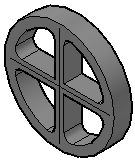
\includegraphics[scale=0.9]{fabanc-c4.png}}
\ffigbox{\caption{绘制$\phi 31$圆柱}\label{fig:fabanc-c5}}{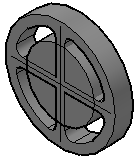
\includegraphics[scale=0.9]{fabanc-c5.png}}
\ffigbox{\caption{减去$\phi 31$圆柱}\label{fig:fabanc-c6}}{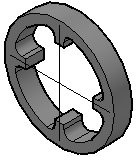
\includegraphics[scale=0.9]{fabanc-c6.png}}
\end{floatrow}
\end{figure}
\newpage
将结果及辅助线一起复制两份备用。
\begin{lstlisting}
|命令: COPY|
|选择对象: 指定对角点: 找到 3 个|
|选择对象:|
|当前设置:  复制模式 = 多个|
|指定基点或 [位移(D)/模式(O)] $<$位移$>$: int 于|
|指定第二个点或 [阵列(A)] $<$使用第一个点作为位移$>$:|
|指定第二个点或 [阵列(A)/退出(E)/放弃(U)] $<$退出$>$:|
|指定第二个点或 [阵列(A)/退出(E)/放弃(U)] $<$退出$>$:|
\end{lstlisting}
\item 绘制$\phi 31$圆柱体,结果如图\ref{fig:fabanc-c5}所示。
\begin{lstlisting}
|命令:  CYLINDER|
|指定底面的中心点或 [三点(3P)/两点(2P)/切点、切点、半径(T)|
|/椭圆(E)]:int 于|
|指定底面半径或 [直径(D)]$<$21.0000$>$: 15.5|
|指定高度或 [两点(2P)/轴端点(A)]$<$-8.0000$>$: |
\end{lstlisting}
\item 减去$\phi 31$圆柱体,结果如图\ref{fig:fabanc-c6}所示。
\begin{lstlisting}
|命令: SUBTRACT|
|选择要从中减去的实体、曲面和面域...|
|选择对象: 找到 1 个|
|选择对象:  选择要减去的实体、曲面和面域...|
|选择对象: 找到 1 个|
|选择对象:|
\end{lstlisting}
\end{procedure}
\subsection{构建$D-D$段实体}
\begin{procedure}
\item 图\ref{fig:fabanc-c4}实体的基础上绘制$\phi 18$圆柱体,结果如图\ref{fig:faband-d1}。
\begin{lstlisting}
|命令:  CYLINDER|
|指定底面的中心点或 [三点(3P)/两点(2P)/切点、切点、半径(T)|
|/椭圆(E)]:int 于|
|指定底面半径或 [直径(D)]$<$15.5000$>$: 9|
|指定高度或 [两点(2P)/轴端点(A)]$<$-8.0000$>$: |
\end{lstlisting}
\item 减去$\phi 18$圆柱体,结果如图\ref{fig:faband-d2}。
\begin{lstlisting}
|命令: SUBTRACT|
|选择要从中减去的实体、曲面和面域...|
|选择对象: 找到 1 个|
|选择对象:  选择要减去的实体、曲面和面域...|
|选择对象: 找到 1 个|
|选择对象:|
\end{lstlisting}
\begin{figure}[htbp]
\centering
\begin{floatrow}[3]
\ffigbox{\caption{绘制$\phi 18$圆柱}\label{fig:faband-d1}}{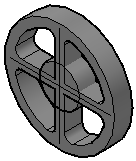
\includegraphics[scale=0.9]{faband-d1.png}}
\ffigbox{\caption{减去$\phi 31$圆柱}\label{fig:faband-d2}}{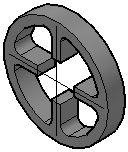
\includegraphics[scale=0.9]{faband-d2.png}}
\ffigbox{\caption{选拉伸面}\label{fig:faband-d3}}{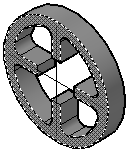
\includegraphics[scale=0.9]{faband-d3.png}}
\end{floatrow}
\end{figure}

\item 拉伸面。

由于图\ref{fig:fabanc-c4}所构建的实体长度比$D-D$段的实体短4mm,所以需要通过拉伸面操作来增加长度。面拉伸操作的启动方法有:
\begin{itemize}
\item 键盘输入SOLIDEDIT,选择【面F】选项中的【拉伸E】选项。
\item 点击【修改】菜单中【实体编辑】子菜单中的【拉伸面】项。
\item 点击【实体编辑】工具栏中的【拉伸面】图标
\includegraphics[scale=0.6]{solideditface.png}
\end{itemize}
用鼠标点击拉伸面图标。
\begin{lstlisting}
|命令: solidedit|
|实体编辑自动检查:  SOLIDCHECK=1|
|输入实体编辑选项 [面(F)/边(E)/体(B)/放弃(U)/退出(X)]|
| $<$退出$>$: \-face|
|输入面编辑选项|
|[拉伸(E)/移动(M)/旋转(R)/偏移(O)/倾斜(T)/删除(D)/复制(C)|
|/颜色(L)/材质(A)/放弃(U)/退出(X)] $<$退出$>$: \_extrude|
\end{lstlisting}
按图\ref{fig:faband-d3}所示方式选择拉伸面。
\begin{lstlisting}
|选择面或 [放弃(U)/删除(R)]: 找到一个面。|
|选择面或 [放弃(U)/删除(R)/全部(ALL)]:|
\end{lstlisting}
指定拉伸参数,并按提示结束命令,结果如图\ref{fig:faband-d4}所示。
\begin{lstlisting}
|指定拉伸高度或 [路径(P)]: 4|
|指定拉伸的倾斜角度 $<$0$>$:|
|已开始实体校验。|
|已完成实体校验。|
|输入面编辑选项|
|[拉伸(E)/移动(M)/旋转(R)/偏移(O)/倾斜(T)/删除(D)/复制(C)|
|/颜色(L)/材质(A)/放弃(U)/退出(X)] $<$退出$>$:|
|实体编辑自动检查:  SOLIDCHECK=1|
|输入实体编辑选项 [面(F)/边(E)/体(B)/放弃(U)/退出(X)]$<$退出$>$:|
\end{lstlisting}
\end{procedure}

\begin{figure}[htbp]
\centering
\begin{floatrow}[3]
\ffigbox{\caption{$D-D段$实体}\label{fig:faband-d4}}{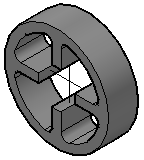
\includegraphics[scale=0.9]{faband-d4.png}}
\ffigbox{\caption{绘制$\phi 8$圆柱}\label{fig:fabane-e1}}{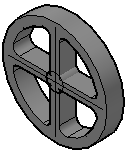
\includegraphics[scale=0.9]{fabane-e1.png}}
\ffigbox{\caption{减去$\phi 8$圆柱}\label{fig:fabane-e2}}{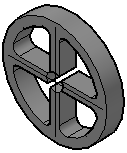
\includegraphics[scale=0.9]{fabane-e2.png}}
\end{floatrow}
\end{figure}
\subsection{构建$E-E$段实体}
\begin{procedure}
\item 图\ref{fig:fabanc-c4}实体的基础上绘制$\phi 8$圆柱体,结果如图\ref{fig:fabane-e1}。
\begin{lstlisting}
|命令:  CYLINDER|
|指定底面的中心点或 [三点(3P)/两点(2P)/切点、切点、半径(T)|
|/椭圆(E)]:int 于|
|指定底面半径或 [直径(D)]$<$9.0000$>$: 8|
|指定高度或 [两点(2P)/轴端点(A)]$<$-8.0000$>$: |
\end{lstlisting}
\item 减去$\phi 18$圆柱体,结果如图\ref{fig:fabane-e2}所示。
\begin{lstlisting}
|命令: SUBTRACT|
|选择要从中减去的实体、曲面和面域...|
|选择对象: 找到 1 个|
|选择对象:  选择要减去的实体、曲面和面域...|
|选择对象: 找到 1 个|
|选择对象:|
\end{lstlisting}
\item 拉伸面。

由于图\ref{fig:fabanc-c4}所构建的实体长度比$E-E$段的实体短长6mm,所以需要通过拉伸面操作来减少长度。操作完成后结果如图\ref{fig:fabane-e3}所示。
\begin{lstlisting}
|命令: solidedit|
|实体编辑自动检查:  SOLIDCHECK=1|
|输入实体编辑选项 [面(F)/边(E)/体(B)/放弃(U)/退出(X)]|
| $<$退出$>$: \-face|
|输入面编辑选项|
|[拉伸(E)/移动(M)/旋转(R)/偏移(O)/倾斜(T)/删除(D)/复制(C)|
|/颜色(L)/材质(A)/放弃(U)/退出(X)] $<$退出$>$: \_extrude|
|选择面或 [放弃(U)/删除(R)]: 找到一个面。|
|选择面或 [放弃(U)/删除(R)/全部(ALL)]:|
|指定拉伸高度或 [路径(P)]: 6|
|指定拉伸的倾斜角度 $<$0$>$:|
|已开始实体校验。|
|已完成实体校验。|
|输入面编辑选项|
|[拉伸(E)/移动(M)/旋转(R)/偏移(O)/倾斜(T)/删除(D)/复制(C)|
|/颜色(L)/材质(A)/放弃(U)/退出(X)] $<$退出$>$:|
|实体编辑自动检查:  SOLIDCHECK=1|
|输入实体编辑选项 [面(F)/边(E)/体(B)/放弃(U)/退出(X)]$<$退出$>$:|
\end{lstlisting}
\begin{figure}[htbp]
\centering
\begin{floatrow}[3]
\ffigbox{\caption{拉伸面结果}\label{fig:fabane-e3}}{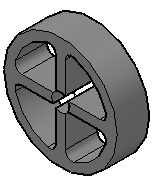
\includegraphics[scale=1.1]{fabane-e3.png}}
\ffigbox{\caption{移动结果}\label{fig:fabane-e4}}{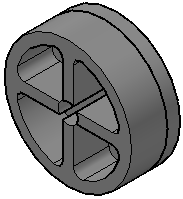
\includegraphics[scale=0.9]{fabane-e4.png}}
\ffigbox{\caption{合并结果}\label{fig:fabane-e5}}{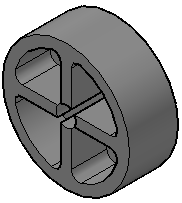
\includegraphics[scale=0.9]{fabane-e5.png}}
\end{floatrow}
\end{figure}
\item 绘制$\phi 50$圆柱体。
\begin{lstlisting}
|命令:  CYLINDER|
|指定底面的中心点或 [三点(3P)/两点(2P)/切点、切点、半径(T)|
|/椭圆(E)]:int 于|
|指定底面半径或 [直径(D)]$<$8.0000$>$: 25|
|指定高度或 [两点(2P)/轴端点(A)]$<$-8.0000$>$:5 |
\end{lstlisting}
\item 将图\ref{fig:fabane-e3}所示的实体移动到$\phi 50$圆柱上,结果如图\ref{fig:fabane-e4}所示。

移动命令的启动方法有:
\begin{itemize}
\item 键盘输入MOVE或M。
\item 点击【修改】菜单中的【移动】项。
\item 点击【修改】工具栏中【移动】图标
\includegraphics[scale=0.6]{move.png}
\end{itemize}
选择图\ref{fig:fabane-e3}实体。
\begin{lstlisting}
|命令:MOVE|
|选择对象: 找到 1 个|
|选择对象:|
\end{lstlisting}
以图\ref{fig:fabane-e3}实体的最右圆心为基点。
\begin{lstlisting}
|指定基点或 [位移(D)] $<$位移$>$:|
\end{lstlisting}
以$\phi 50$圆柱体最左圆心为目标点。
\begin{lstlisting}
|指定第二个点或 $<$使用第一个点作为位移$>$:
\end{lstlisting}
\item 合并实体,结果如\ref{fig:fabane-e5}所示。
\begin{lstlisting}
|命令: UNION|
|选择对象: 找到 1 个|
|选择对象: 找到 1 个,总计 2 个|
|选择对象:|
\end{lstlisting}
\end{procedure}

\subsection{构建$F-F$段实体}
\begin{procedure}
\item 以图\ref{fig:fabanc-c2}所示的十字体辅助线交点为圆心,绘制$\phi 11$圆柱体,结果如图\ref{fig:fabanf-f1}所示。
\begin{lstlisting}
|命令:  CYLINDER|
|指定底面的中心点或 [三点(3P)/两点(2P)/切点、切点、半径(T)|
|/椭圆(E)]:int 于|
|指定底面半径或 [直径(D)]$<$25.0000$>$: 5.5|
|指定高度或 [两点(2P)/轴端点(A)]$<$-5.0000$>$:-8 |
\end{lstlisting}
\item 合并实体,结果如图\ref{fig:fabanf-f2}所示。
\begin{lstlisting}
|命令: UNION|
|选择对象: 找到 1 个|
|选择对象: 找到 1 个,总计 2 个|
|选择对象:|
\end{lstlisting}
\begin{figure}[htbp]
\centering
\begin{floatrow}[3]
\ffigbox{\caption{绘制$\phi 11$圆柱}\label{fig:fabanf-f1}}{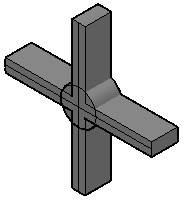
\includegraphics[scale=0.9]{fabanf-f1.png}}
\ffigbox{\caption{合并结果}\label{fig:fabanf-f2}}{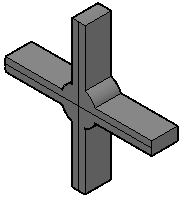
\includegraphics[scale=0.9]{fabanf-f2.png}}
\ffigbox{\caption{拉伸面结果}\label{fig:fabanf-f3}}{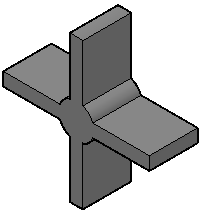
\includegraphics[scale=0.9]{fabanf-f3.png}}
\end{floatrow}
\end{figure}
\item 拉伸面。

由于图\ref{fig:fabanc-c2}的实体比$F-F$段的实体短7mm,故进行面拉伸操作,结果如图\ref{fig:fabanf-f3}。
\begin{lstlisting}
|命令: solidedit|
|实体编辑自动检查:  SOLIDCHECK=1|
|输入实体编辑选项 [面(F)/边(E)/体(B)/放弃(U)/退出(X)]|
| $<$退出$>$: \-face|
|输入面编辑选项|
|[拉伸(E)/移动(M)/旋转(R)/偏移(O)/倾斜(T)/删除(D)/复制(C)|
|/颜色(L)/材质(A)/放弃(U)/退出(X)] $<$退出$>$: \_extrude|
|选择面或 [放弃(U)/删除(R)]: 找到一个面。|
|选择面或 [放弃(U)/删除(R)/全部(ALL)]:|
|指定拉伸高度或 [路径(P)]: 7|
|指定拉伸的倾斜角度 $<$0$>$:|
|输入面编辑选项|
|[拉伸(E)/移动(M)/旋转(R)/偏移(O)/倾斜(T)/删除(D)/复制(C)|
|/颜色(L)/材质(A)/放弃(U)/退出(X)] $<$退出$>$:|
|实体编辑自动检查:  SOLIDCHECK=1|
|输入实体编辑选项 [面(F)/边(E)/体(B)/放弃(U)/退出(X)]$<$退出$>$:|
\end{lstlisting}
\item 绘制$R1$圆角边,结果如图\ref{fig:fabanf-f4}。
\begin{lstlisting}
|命令:  FILLETEDGE|
|半径 = 3.0000|
|选择边或 [链(C)/环(L)/半径(R)]: r|
|输入圆角半径或 [表达式(E)] $<$3.0000$>$: 1|
|选择边或 [链(C)/环(L)/半径(R)]:|
|选择边或 [链(C)/环(L)/半径(R)]:|
|选择边或 [链(C)/环(L)/半径(R)]:|
|选择边或 [链(C)/环(L)/半径(R)]:|
|选择边或 [链(C)/环(L)/半径(R)]:|
|选择边或 [链(C)/环(L)/半径(R)]:|
|选择边或 [链(C)/环(L)/半径(R)]:|
|选择边或 [链(C)/环(L)/半径(R)]:|
|选择边或 [链(C)/环(L)/半径(R)]:|
|选择边或 [链(C)/环(L)/半径(R)]:|
|选择边或 [链(C)/环(L)/半径(R)]:|
|选择边或 [链(C)/环(L)/半径(R)]:|
|选择边或 [链(C)/环(L)/半径(R)]:|
|选择边或 [链(C)/环(L)/半径(R)]:|
|选择边或 [链(C)/环(L)/半径(R)]:|
|选择边或 [链(C)/环(L)/半径(R)]:|
|选择边或 [链(C)/环(L)/半径(R)]:|
|选择边或 [链(C)/环(L)/半径(R)]:|
|已选定 16 个边用于圆角。|
|按 Enter 键接受圆角或 [半径(R)]:|
\end{lstlisting}
\begin{figure}[htbp]
\centering
\begin{floatrow}[3]
\ffigbox{\caption{绘制$R1$圆角}\label{fig:fabanf-f4}}{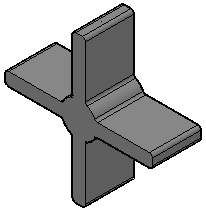
\includegraphics[scale=0.9]{fabanf-f4.png}}
\ffigbox{\caption{倒边角}\label{fig:fabanf-f5}}{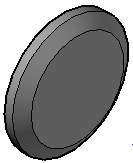
\includegraphics[scale=1]{fabanf-f5.png}}
\ffigbox{\caption{拉伸面结果}\label{fig:fabanf-f6}}{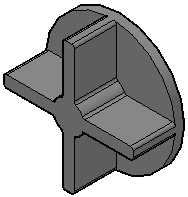
\includegraphics[scale=0.9]{fabanf-f6.png}}
\end{floatrow}
\end{figure}
\item 绘制$\phi 46$圆柱体
\begin{lstlisting}
|命令:  CYLINDER|
|指定底面的中心点或 [三点(3P)/两点(2P)/切点、切点、半径(T)|
|/椭圆(E)]:int 于|
|指定底面半径或 [直径(D)]$<$5.5000$>$: 23|
|指定高度或 [两点(2P)/轴端点(A)]$<$-8.0000$>$:6 |
\end{lstlisting}
\item 倒$30^o$边角,东南等轴测结果如图\ref{fig:fabanf-f5}所示。
\begin{lstlisting}
|命令: CHAMFER|
|(“修剪”模式) 当前倒角距离 1 = 0.0000,距离 2 = 0.0000|
|选择第一条直线或 [放弃(U)/多段线(P)/距离(D)/角度(A)/修剪(T)|
|/方式(E)/多个(M)]:|
|基面选择...|
|输入曲面选择选项 [下一个(N)/当前(OK)] $<$当前(OK)$>$:|
|指定基面倒角距离或 [表达式(E)]: 4.5|
|指定其他曲面倒角距离或 [表达式(E)] $<$4.5000$>$: 3|
|选择边或 [环(L)]:|
|选择边或 [环(L)]:|
\end{lstlisting}
\item 将图\ref{fig:fabanf-f4}实体移动到图\ref{fig:fabanf-f5}的实体上。
\begin{lstlisting}
|命令:MOVE|
|选择对象: 找到 1 个|
|选择对象:|
|指定基点或 [位移(D)] $<$位移$>$:|
|指定第二个点或 $<$使用第一个点作为位移$>$:
\end{lstlisting}
\item 合并实体,结果如图\ref{fig:fabanf-f6}所示。
\begin{lstlisting}
|命令: UNION|
|选择对象: 找到 1 个|
|选择对象: 找到 1 个,总计 2 个|
|选择对象:|
\end{lstlisting}
\end{procedure}
\subsection{组合各部件}
\begin{procedure}
\item 组合$E-E$段和$F-F$段,结果如图所示。
\begin{lstlisting}
|命令:MOVE|
|选择对象: 找到 1 个|
|选择对象:|
|指定基点或 [位移(D)] $<$位移$>$:|
|指定第二个点或 $<$使用第一个点作为位移$>$:
\end{lstlisting}
\begin{figure}[htbp]
\centering
\begin{floatrow}[3]
\ffigbox{\caption{组合E段和F段}\label{fig:faban1}}{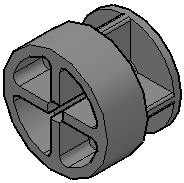
\includegraphics[scale=0.7]{faban1.png}}
\ffigbox{\caption{组合D段}\label{fig:faban2}}{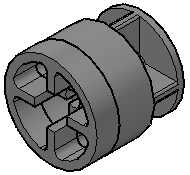
\includegraphics[scale=0.7]{faban2.png}}
\ffigbox{\caption{组合C段}\label{fig:faban3}}{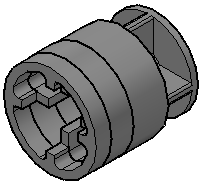
\includegraphics[scale=0.7]{faban3.png}}
\end{floatrow}
\end{figure}
\item 组合D段。
\begin{lstlisting}
|命令:MOVE|
|选择对象: 找到 1 个|
|选择对象:|
|指定基点或 [位移(D)] $<$位移$>$:|
|指定第二个点或 $<$使用第一个点作为位移$>$:
\end{lstlisting}
\item 组合C段。
\begin{lstlisting}
|命令:MOVE|
|选择对象: 找到 1 个|
|选择对象:|
|指定基点或 [位移(D)] $<$位移$>$:|
|指定第二个点或 $<$使用第一个点作为位移$>$:
\end{lstlisting}
\newpage
\item 组合B段。
\begin{lstlisting}
|命令:MOVE|
|选择对象: 找到 1 个|
|选择对象:|
|指定基点或 [位移(D)] $<$位移$>$:|
|指定第二个点或 $<$使用第一个点作为位移$>$:
\end{lstlisting}
\begin{figure}[htbp]
\centering
\begin{floatrow}[3]
\ffigbox{\caption{组合B段}\label{fig:faban4}}{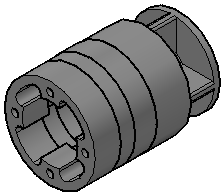
\includegraphics[scale=0.6]{faban4.png}}
\ffigbox{\caption{西南等轴测}\label{fig:faban5}}{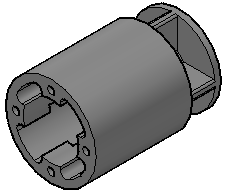
\includegraphics[scale=0.6]{faban5.png}}
\ffigbox{\caption{东南等轴测}\label{fig:faban6}}{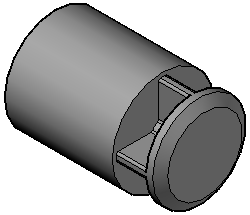
\includegraphics[scale=0.6]{faban6.png}}
\end{floatrow}
\end{figure}
\begin{lstlisting}
|命令: UNION|
|选择对象:指定对角点: 找到 5 个|
|选择对象:|
\end{lstlisting}
\end{procedure}
\endinput
